\capitulo{3}{Conceptos teóricos}

Este apartado va a explicar los conceptos teóricos necesarios para poder entender el proyecto.

\section{Minería de Datos}
\begin{quote}
Es conocida la frase <<los datos en bruto raramente son beneficiosos directamente>>. Pueden tener valor, ya que podemos extraer información útil para la toma de decisiones o exploración, y también para la compresión del fenómeno dominante en el conjunto de datos~\cite{mineria}.
\end{quote}

La finalidad de esto es descubrir unos patrones, una similitud o una propensión que expliquen el comportamiento de los datos. Para hacer esto utiliza los métodos de la inteligencia artificial y estadística.
El objetivo del proceso de minería de datos consiste en extraer información de un conjunto de datos, luego se interpreta esta información para un uso posterior~\cite{wiki:datamining}.

La minería de datos está basada en el aprendizaje automático, para ello se considera un conjunto con $n$ muestras y se intenta predecir las propiedades de los datos desconocidos. Podemos separar los problemas de aprendizaje principalmente en dos~\cite{scikitlearn2}:
	\begin{itemize}
		\item Aprendizaje supervisado: Consiste en que a partir de un conjunto de datos, hacer predicciones basadas en el comportamiento o las características de dichos datos. Nos permite buscar patrones en datos. Dos de las tareas más comunes del aprendizaje supervisado son la clasificación y la regresión:
		
		\begin{itemize}
		 	\item Clasificación: El programa debe aprender a predecir en que categoría o clase irán los nuevos datos, según las nuevas observaciones, por ejemplo, predecir si el precio de una acción bajará o subirá.
		 	\item Regresión: El programa debe predecir el valor de una variable de respuesta continua, por ejemplo, predecir las ventas de un nuevo producto.
		\end{itemize}
		
		\item Aprendizaje no supervisado: Usa datos que no están etiquetados. El objetivo es explorarlos para encontrar alguna forma de organizarlos.
	\end{itemize}

La minería de datos está incluida en el proceso de KDD (Knowledge Discovery in Databases, Descubrimiento del conocimiento en bases de datos) Este proceso tiene una secuencia de pasos~\cite{mineria_KDD}:

\begin{enumerate}[1.]
	\item Limpieza de datos. Eliminación del ruido y la inconsistencia de los datos.
	\item Integración de los datos. Múltiples fuentes de datos son combinadas.
	\item Selección de datos. Los datos relevantes para la tarea de análisis se recuperan de la base de datos.
	\item Transformación de datos. Los datos son transformados y se consolidan como apropiados para la minería mediante la realización de operaciones simétricas o de agregación.
	\item Minería de datos. Es un proceso esencial donde los métodos de inteligencia son aplicados a la extracción de patrones.
	\item Evaluación de patrones. Identificar los patrones que de verdad son interesantes, que representan el conocimiento basado en medidas de interés.
	\item Presentación del conocimiento. Representación visual de los resultados obtenidos.
\end{enumerate}

Aunque el proceso de la minería de datos consta de más etapas nosotros nos centraremos en 4 etapas~\cite{datamining}:
\begin{itemize}
	\item Determinación de los objetivos: Se tratan los objetivos que quiere conseguir el cliente bajo un asesor especialista en minería de datos.
	\item Preprocesamiento de los datos: Es la etapa que más tiempo se tarda en realizar el proceso. Se seleccionan, limpian, enriquecen, reducen y transforman las bases de datos.
	\item Determinación del modelo: Se lleva a cabo un estudio estadístico de los datos, más tarde se hace una visualización gráfica para una primera aproximación. Según los objetivos que se habían propuesto se pueden usar diferentes algoritmos de la Inteligencia Artificial.
	\item  Análisis de los resultados: Se comprueban si los datos obtenidos tienen coherencia, después se comparan con los obtenidos en los estudios estadísticos y la visualización gráfica. El cliente es el que ve si los datos le aportan nuevo conocimiento que le permita considerar sus decisiones.
\end{itemize}

\section{Multi-Label}
Al principio el aprendizaje supervisado trataba con el análisis de datos de Single-Label donde los ejemplos de entrenamiento son asociados con un Single-Label de un conjunto que no tiene nada en común con otros conjuntos. Sin embargo, los ejemplos de entrenamiento a veces se pueden asociar a un conjunto de labels, a los que llamaremos Multi-Label~\cite{multilabel2}.

La clasificación Single-Label y Multi-Label son unas tareas que se pueden resolver con distintas técnicas de minería de datos, la cual nos permite que a partir de un conjunto de instancias de entrenamiento, podamos determinar a través de unos atributos esenciales de dichas instancias, crear unas reglas que posteriormente se usarán para clasificar nuevas instancias~\cite{multilabel}. Como por ejemplo en el etiquetado de imágenes: en el que una imagen puede tener a la vez las etiquetas <<árbol>>, <<montaña>> y <<mar>>.   

\section{\textit{Ensemble}}
Un \textit{ensemble} es un esquema de combinación de clasificadores base con los que obtenemos unas predicciones individuales. El éxito de un \textit{ensemble} requiere tanto exactitud como diversidad de sus clasificadores base. La diversidad representa como de diferente son las predicciones de los clasificadores base. Si los clasificadores base siempre están de acuerdo no habría diferencia entre usar sólo un clasificador base o varios combinado por un método de \textit{ensemble}. Entonces la ventaja de usar un \textit{ensemble} de clasificadores base consiste en la posibilidad que algunos de ellos pueden corregir una predicción incorrecta de otros, por lo que cuantos más clasificadores tengamos más precisas serán las predicciones. 

Es normal obtener estos clasificadores base en un \textit{ensemble} usando el mismo algoritmo, así que en esta situación el proceso de entrenamiento realizado por el \textit{ensemble} es la principal fuente de diversidad. La diversidad de Bagging~\cite{bagging} proviene de elegir al azar diferentes instancias para entrenar a cada clasificador de base. El método Random Subspaces~\cite{randomsubspace} elige diferentes subconjuntos de atributos para entrenar a cada clasificador base. Boosting~\cite{boosting} entrena de forma iterativa el conjunto de clasificadores base, modificando los pesos de las instancias para entrenar al clasificador actual. Estos nuevos pesos se calculan a partir del error de entrenamiento en el clasificador base anterior, por lo que cada nuevo clasificador de base llega más especializado en instancias que han sido mal clasificados antes. A veces los clasificadores base son muy estables y el  algoritmo de entrenamiento del \textit{ensemble} no es suficiente para proporcionar el nivel deseado de diversidad~\cite{disturbingneighbors}.

Los métodos de \textit{ensembles} combinan las predicciones de unos estimadores base, que están construidos mediante un algoritmo de aprendizaje para mejorar la solidez de un solo estimador~\cite{ensemble}.
Se distinguen dos clases de métodos de \textit{ensembles}:
	\begin{itemize}
		\item En los métodos de Bagging~\cite{bagging}, se construyen varios estimadores de forma independiente y luego se calcula su promedio para las predicciones.
		\item En los métodos de Boosting~\cite{boosting}, se construyen los estimadores secuencialmente y se trata de reducir el sesgo del estimador combinado. 
	\end{itemize}
	
Podemos ver un ejemplo de un ensemble de clasificadores en la siguiente figura~\ref{fig:Ensembles}~\cite{figensemble}.

\begin{figure}
\centering
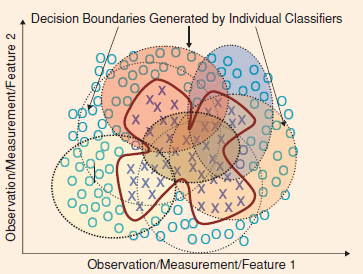
\includegraphics[width=0.95\textwidth]{Ensembles}
\caption{Ensemble de clasificadores que abarca un espacio de decisión}
\label{fig:Ensembles}
\end{figure}

\section{Disturbing Neighbors}

Los Disturbing Neighbors (DN) o vecinos molestones se han utilizado con éxito para mejorar la diversidad en los bosques~\cite{disturbingneighbors}.

El método DN trabaja en cada clasificador base de la siguiente manera:
\begin{itemize}
    \item $m$ instancias son seleccionadas aleatoriamente de el conjunto de datos de entrenamiento para construir un clasificador 1-NN. El valor $m$ suelen ser valores muy pequeños.
    \item Las dimensiones para calcular la distancia euclidea en el clasificador 1-NN, también se seleccionan. Como mínimo se seleccionan el 50\% de los atributos.
    \item Luego $m+1$ nuevas características son añadidas al conjunto de entrenamiento. Una de las características adicionales es la clase predicha por el clasificador 1-NN para cada instancia \textbf{x}, y las otras $m$ son características booleanas, todos los valores falsos excepto uno corresponden al vecino más cercano para esa instancia.
    \item El clasificador base está entrenado usando las características originales mas las nuevas $m+1$ características. 
\end{itemize}
Por lo tanto, el proceso normal de entrenamiento de los clasificadores base se altera añadiendo estas nuevas características del clasificador 1-NN. Es por eso que el método se llama vecinos molestones. La aleatoriedad aumenta la diversidad y se debe a:
\begin{itemize}
\item Los vecinos utilizados en cada clasificador 1-NN se seleccionan aleatoriamente. Por lo tanto, sus predicciones y las características booleanas son diferentes para cada clasificador base.
\item Las dimensiones utilizadas para calcular las distancias euclidianas también se eligen de forma aleatoria, así que si dos clasificadores básicos tienen al menos los mismos m vecinos, las predicciones 1-NN y las características booleanas podrían ser diferentes.
\end{itemize}

En resumen, Disturbing Neighbors es un método para alterar el proceso de entrenamiento normal de los clasificadores base en un \textit{ensemble}, mejorando su diversidad y mejorando la precisión general del \textit{ensemble}.

\section{Random Oracles}

Random Oracles son mini-ensembles formados por dos o más modelos, pueden usarse como modelos base para otros métodos \textit{ensemble}. El objetivo de usar Random Oracles es tener más diversidad entre los modelos base que forman un \textit{ensemble}~\cite{randomoracles}.

Dado un método base, el entrenamiento de un Random Oracle consiste en:
\begin{itemize}

	\item Seleccionar aleatoriamente un Random Oracle.
	\item Dividir los datos de entrenamiento en dos o más subconjuntos usando el Random Oracle.
	\item Para cada subconjunto de datos de entrenamiento, se construye un modelo (en nuestro caso un árbol, aunque se pueden construir otros modelos). El modelo Random Oracle está formado por los modelos cada subconjunto y el propio oráculo.
\end{itemize}
La predicción del test de una instancia se realiza de la siguiente manera: 
\begin{itemize}
	\item Usa el Random Oracle para seleccionar uno de los dos o más modelos.
	\item Devuelve la predicción obtenida por el modelo seleccionado.
\end{itemize}

Se pueden considerar diferentes tipos de Oracles. En este trabajo, se utiliza el Linear Random Oracle. Este oráculo divide el espacio en dos o más subespacios utilizando un hiperplano. Para construir el oráculo, dos o más objetos de entrenamiento diferentes se seleccionan aleatoriamente, cada objeto de entrenamiento restante se asigna al subespacio del objeto de entrenamiento seleccionado que está más cerca.

\section{Rotation Forest}

Rotation Forest, tiene como objetivo construir clasificadores precisos y diversos. La heurística principal consiste en aplicar la extracción de características a subconjuntos de características y reconstruir un conjunto completo de características para cada clasificador en el conjunto. En el artículo original se utiliza el Análisis de Componentes Principales (PCA)~\cite{rotationforest}.

Para construir el clasificador se siguen los siguientes pasos:
\begin{itemize}
	\item Dividir los atributos del conjunto de datos en $K$ subconjuntos. Para maximizar la diversidad se eligen subconjuntos disjuntos.
	\item De las clases se seleccionan las que son distintas, y de estas se selecciona una muestra, en nuestro caso la muestra tiene un tamaño del 80\%.
	\item Para cada subconjunto se selecciona aleatoriamente una muestra, por defecto con un tamaño del 75\%. Se ejecuta PCA sobre cada una de las muestras.
	\item Después de todos los pasos anteriores, para predecir se hace el \texttt{predict} del estimador base.
\end{itemize}

De esta forma, se construyen clasificadores individuales precisos.